\chapter{Self-Healing Architecture} \label{ch:selfHelingArchitecture}

\textbf{2.1. Version One (Self-Healing Loop):\\}

Model proposed by Kephart and Chess. The different stages of self-healing loops are: \\


\begin{figure}[H]
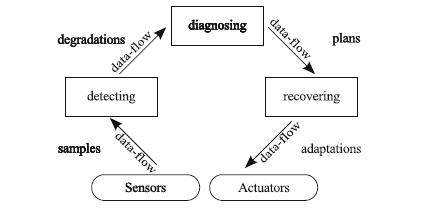
\includegraphics[width=5in]{img/SelfHealingStagesHarald}
\caption{The different stages of self-healing loops are:}
\end{figure}

\textit{2.1.1.Detect:} This stage filters any suspicious status data got from tests and reports recognized degradation. This stage is similar to Monitoring, which observes the behaviour of a system and the values of the specific suspicious parameters(called indicators)\\

\textit{2.1.2.Diagnose:} This stage incorporates root cause analysis, and computes a proper recuperation arrangement with the assistance of a policy base.(Self-healing policies).This determines whether a detected deviation of a set of detected deviations could be characterized as a fault.\\

\textit{2.1.3.Recovery:} This stage deliberately applies the arranged adjustments meeting the imperatives of the framework abilities and maintains a strategic distance from any unpredictable side effects.\cite{Harald:SelfHealingSurvey:2011}.   

\textbf{2.2.Version Two (Self-Healing Loop):\\}\\

\begin{figure}[H]
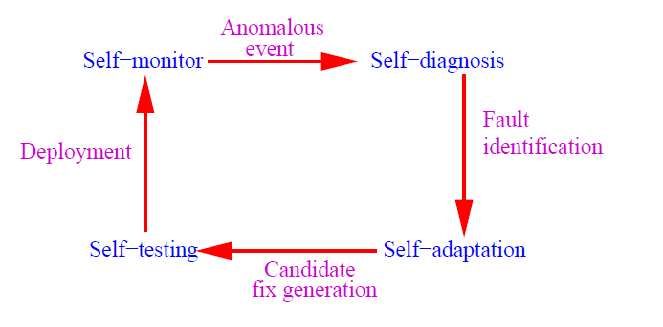
\includegraphics[width=5in]{img/SelfHealingStagesKeromytis}
\caption{The different stages of self-healing loops are:}
\end{figure}

The general architecture of a self-healing system can be divided in to four states: \\

\textit{2.2.1.Self-monitor:} In this state the system monitors for any abnormal or unexpected behaviour (Anomalous Event)\\

\textit{2.2.2.Self-diagnosis:} If such behaviours are detected, the system enters the self-diagnosis mode, where the main task is to fetch as much as information with respect to the specific fault that has been detected. The main goal of this identification stage is to detect the type of fault, the input/events which led the fault, the exact region in the code where the fault occurred and useful strategies for fixing the fault. (Fault Identification).\\

\textit{2.2.3.Self-adaption:} After identification the system needs to create one or more possible fixes with respect to the particular fault. Some of the important strategies to fix software faults include snapshot-rollback, input filtering, increased monitoring, isolation for the vulnerable process and selective application of any runtime protection mechanism.\\

\textit{2.2.4.Self-testing:} Depending on the efficiency of anyone of the fault-identification techniques. (e.g., in terms of side effects or performance degradation), we choose one of them. If an appropriate fix is produced the system is upgraded to the normalcy accordingly. The most important mechanisms for this are established patch-management and configuration-management. After figuring the best possible solutions.
\cite{Keromytis:SelfHealingSurvey:2011}.\\

\textbf{2.3.Version Three (Self-Healing Loop):\\}

The third version of the Self-Healing Loop defined by Ghosh et al. consists of three steps:   a) maintenance of the system health, (b) detection of system failure and (c) system recovery process. The Self-Healing Loop Is defined in the figure:

\begin{figure}[H]
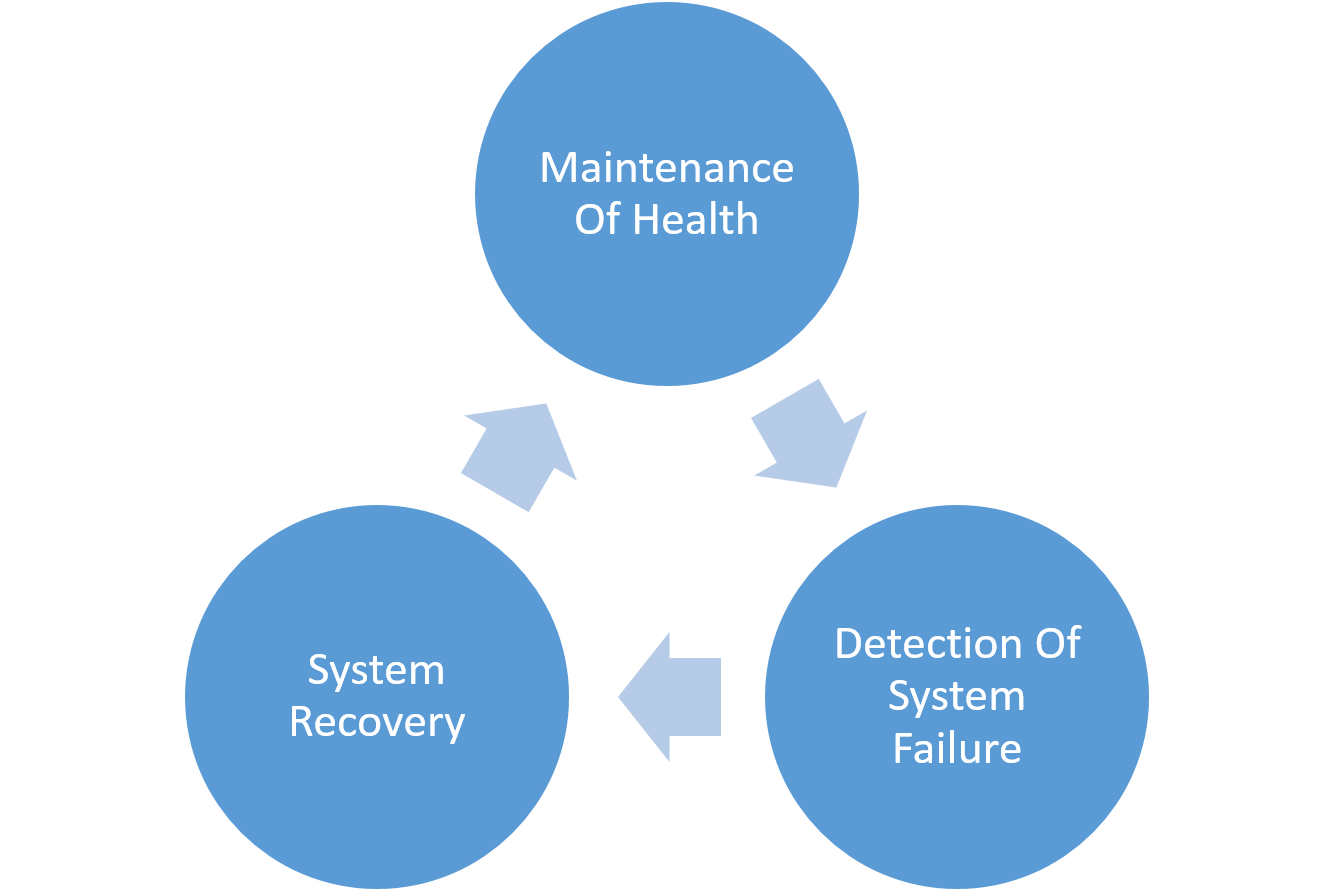
\includegraphics[width=5in]{img/SelfHealingStagesGhoshetal}
\caption{Steps Taken By A Self-Healing System When A Fault Occurs:}
\end{figure}

\textit{2.3.1.System Maintenance Of Health:}
The system should check for faults periodically to
continue monitoring its health.The various strategies that can be used to maintain the system health are:
1. Maintaining Redundancy
2. Maintenance By Probing
3. System Monitoring Model
4. Maintaining Diversity
5. Performance Log Analysis\\

\textit{2.3.2.Detection Of System Failure:}
Failure detection is another major area of research.Several approaches have been adopted
to detect non-self or abnormality in the functioning of the system are:
1. Missing Component/Message Response
2. System Monitoring Model
3. Identification Of Foreign Element\\

\textit{2.3.3.System Recovery:}
System recovery involves mechanisms to transform a system from an unhealthy state to a healthy state. 
This various redundancy techniques are:

1. Redundancy Techniques
2. Architectural Models And Repair Plans
3. Byzantine Agreement And Voting
4. Other Non-Traditional Methods
\cite{Ghosh:SelfHealingSurvey:2007}.\\
